\section{Realisierungs Methoden}
\subsection{ROM}
Mit einem ROM lassen sich sich kombinatorische Schaltungen in Form einer Look up Table realisieren.\\
\begin{itemize}
	\setlength{\itemsep}{1pt}
  \setlength{\parskip}{0pt}
  \setlength{\parsep}{0pt}
  
	\item Eingangsvariablen = Adresse\\
	\item Speicherwert = Ausgang (programmierbar)\\
\end{itemize}

\begin{itemize}
	\setlength{\itemsep}{1pt}
  \setlength{\parskip}{0pt}
  \setlength{\parsep}{0pt}
  
	\item ROM $\rightarrow$ Bei der Herstellung programmierter Speicher\\
	\item PROM $\rightarrow$ Programmierbares ROM (Fuses)\\
	\item EPROM $\rightarrow$ L"oschbares PROM (UV Licht)\\
	\item EEPROM $\rightarrow$ Elektrisch l"oschbares PROM\\
	\item Flash $\rightarrow$ Blockweise beschreibbares EEPROM (schneller)\\
\end{itemize}

\subsection{PLD}
Programmierbares Device aus AND und OR-Matrix, mindestens eine Matrix programmierbar.
\begin{itemize}
	\setlength{\itemsep}{1pt}
  \setlength{\parskip}{0pt}
  \setlength{\parsep}{0pt}
  
	\item PAL $\rightarrow$ OR-Matrix fest, AND-Matrix programmierbar, Fuses\\
	\item PLA $\rightarrow$ OR und AND Matrix frei programmierbar, Fuses\\
	\item GAL $\rightarrow$ Wie PLA plus programmierbare Ausgangsnetzwerke (Tristate), EEPROM\\
\end{itemize}
F�r Funktionen die als DNF vorliegen geeignet, heute gr�sstenteils von CPLD und FPGA verdr�ngt.\\

\subsection{CPLD}
\begin{itemize}
	\setlength{\itemsep}{1pt}
  \setlength{\parskip}{0pt}
  \setlength{\parsep}{0pt}
  
	\item Verbund PLD Makrozellen die mit Bussen verbunden sind, Speicherung der Konfiguration in Flash.\\
	\item	Durch regelm"assige Struktur sind Signallaufzeiten vorhersagbar.\\
	\item Wegen grosser Zahl an Logikbl�cken sehr gut f�r parallele Prozesse geeignet.\\
\end{itemize}

\subsection{FPGA}
2D-Array von Logikbl"ocken, die �ber Routing Kanal und Schaltmatrizen miteinander und mit I/O verbunden werden.\\
\begin{itemize}
	\setlength{\itemsep}{1pt}
  \setlength{\parskip}{0pt}
  \setlength{\parsep}{0pt}
  
	\item Logikblock (LogicCell) $\rightarrow$ Lookuptable mit D-FlipFlop, kann beliebige Funktionen ausf"uhren
	\item Schaltmatrizen $\rightarrow$ programmierbare Verbindungen
	\item Makrozellen $\rightarrow$ Feste Funktionen z.B. Memory, Clock Managment...
\end{itemize}
Die Konfiguration wird im RAM gespeichert (fl"uchtig). D.h. bei jedem Boot muss der Code von einem Festspeicher geladen werden.\\

\subsection{Xilinx Spartan 3}
\begin{itemize}
	\setlength{\itemsep}{1pt}
  \setlength{\parskip}{0pt}
  \setlength{\parsep}{0pt}

	\item Logic Cell (LC): Kleinste Einheit, enth"alt LUT mit 4 Eing"angen und eime D-FlipFlop. LUT kann als 16x1 bit SRAM oder Schieberegister 		konfiguriert werden. Zus"atzlich pro LC CarryLogic und MUX.
	\item Slice: 1Slice = 2 Logic Cell
	\item Configurable logic bloc (CLB): 1 CLB = 4 Slices = 8 Locic Cells. \\
	Inerhalb dieser Einheit existieren spezifische Verbindungsstrukturen.
\end{itemize}

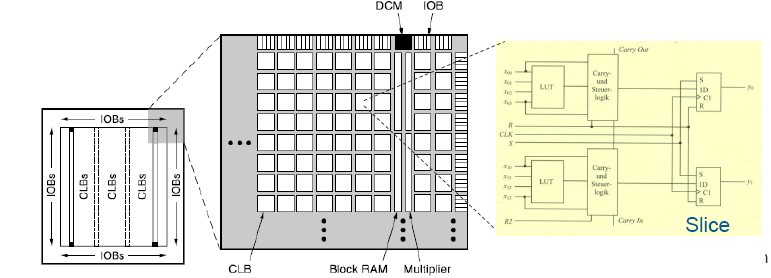
\includegraphics[width=0.8\textwidth]{pics/fpgastruct}


\subsection{Semicustom IC}
\begin{itemize}
	\setlength{\itemsep}{1pt}
  \setlength{\parskip}{0pt}
  \setlength{\parsep}{0pt}
  
	\item Mikrozellen aus p- und n-FETs werden durch Verdrahtung zu Gates.\\
	\item Gates k"onnen durch Verdrahtungskan"ale verbunden werden.\\
	\item Standardfunktionen k"onnen mit IP-Cores implementiert werden.\\
\end{itemize}	
	
\subsection{Fullcustom IC}
V�llig kundenspezifische ICs, oft werden IP-Cores f�r Standardfunktionen verwendet. Digitale und analoge Komponenten auf einem IC m�glich. Voll auf Anwendung anpassbare Eigenschaften (Stromverbrauch, Gr"osse, Geschwindigkeit etc.).\\

\subsection{Vergeichstabelle}

\begin{center}
	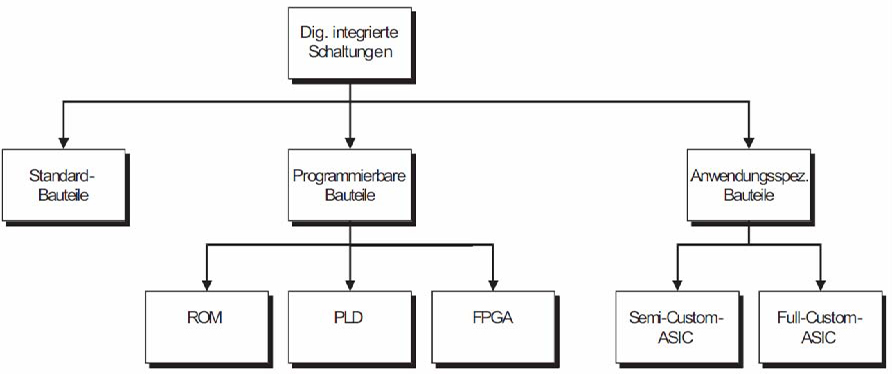
\includegraphics[width=0.60\textwidth]{pics/devicecomparetables}
	
	\begin{tabular}{|l|c|c|c|c|c|c|}
		\hline
		Kriterien & Standard Bauteile & ROM & PLD & FPGA & Semicustom & Fullcustom \\
		\hline
		Machbarkeit & ++ & - - & - - & + & + & +++ \\
		\hline
		Zeit Realisiertung & + & ++ & ++ & ++ & - & - - \\
		\hline
		Iterationszeit & - & ++ & ++ & ++ & - & - - \\
		\hline
		NRE & ++ & + & + & + & - & - - -\\
		\hline
		St"uckpreis & - - & + & + & - & + & +++ \\
		\hline
	\end{tabular}
\end{center}
	